

\tikzset{every picture/.style={line width=0.75pt}} %set default line width to 0.75pt        

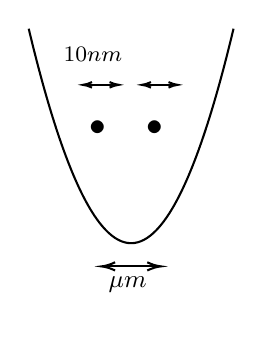
\begin{tikzpicture}[x=0.75pt,y=0.75pt,yscale=-1,xscale=1]
%uncomment if require: \path (0,146); %set diagram left start at 0, and has height of 146

% Plotting does not support converting to Tikz
%Shape: Parabola [id:dp41738409227180906] 
\draw   (5.94,4.49) .. controls (38.83,142.27) and (71.72,142.27) .. (104.61,4.49) ;
%Straight Lines [id:da018467321466964504] 
\draw    (43,119) -- (67.61,119) ;
\draw [shift={(69.61,119)}, rotate = 180] [color={rgb, 255:red, 0; green, 0; blue, 0 }  ][line width=0.75]    (6.56,-1.97) .. controls (4.17,-0.84) and (1.99,-0.18) .. (0,0) .. controls (1.99,0.18) and (4.17,0.84) .. (6.56,1.97)   ;
\draw [shift={(41,119)}, rotate = 0] [color={rgb, 255:red, 0; green, 0; blue, 0 }  ][line width=0.75]    (6.56,-1.97) .. controls (4.17,-0.84) and (1.99,-0.18) .. (0,0) .. controls (1.99,0.18) and (4.17,0.84) .. (6.56,1.97)   ;
%Straight Lines [id:da7958539164071118] 
\draw    (34.07,31.53) -- (47.27,31.53) ;
\draw [shift={(49.27,31.53)}, rotate = 180] [color={rgb, 255:red, 0; green, 0; blue, 0 }  ][line width=0.75]    (4.37,-1.32) .. controls (2.78,-0.56) and (1.32,-0.12) .. (0,0) .. controls (1.32,0.12) and (2.78,0.56) .. (4.37,1.32)   ;
\draw [shift={(32.07,31.53)}, rotate = 0] [color={rgb, 255:red, 0; green, 0; blue, 0 }  ][line width=0.75]    (4.37,-1.32) .. controls (2.78,-0.56) and (1.32,-0.12) .. (0,0) .. controls (1.32,0.12) and (2.78,0.56) .. (4.37,1.32)   ;
%Straight Lines [id:da6691157755991864] 
\draw    (62.47,31.53) -- (75.67,31.53) ;
\draw [shift={(77.67,31.53)}, rotate = 180] [color={rgb, 255:red, 0; green, 0; blue, 0 }  ][line width=0.75]    (4.37,-1.32) .. controls (2.78,-0.56) and (1.32,-0.12) .. (0,0) .. controls (1.32,0.12) and (2.78,0.56) .. (4.37,1.32)   ;
\draw [shift={(60.47,31.53)}, rotate = 0] [color={rgb, 255:red, 0; green, 0; blue, 0 }  ][line width=0.75]    (4.37,-1.32) .. controls (2.78,-0.56) and (1.32,-0.12) .. (0,0) .. controls (1.32,0.12) and (2.78,0.56) .. (4.37,1.32)   ;

% Text Node
\draw (33.8,47.27) node [anchor=north west][inner sep=0.75pt]  [font=\large]  {$\bullet $};
% Text Node
\draw (43,122.4) node [anchor=north west][inner sep=0.75pt]  [font=\small]  {$\mu m$};
% Text Node
\draw (21.27,12.13) node [anchor=north west][inner sep=0.75pt]  [font=\footnotesize]  {$10nm$};
% Text Node
\draw (61.4,47.27) node [anchor=north west][inner sep=0.75pt]  [font=\large]  {$\bullet $};


\end{tikzpicture}
